\documentclass[aspectratio=169, 10pt]{beamer}

%--- Packages ---
\usepackage[utf8]{inputenc}
\usepackage{tikz}
\usepackage{pgfplots}
\usepackage{booktabs}
\usepackage{amsmath}
\usepackage{xcolor}

%--- Theme Settings ---
\usetheme{Madrid}
\usecolortheme{beaver} % Red/Grey theme often fits Econ
\usefonttheme{professionalfonts}

%--- Custom Commands for Graphing ---
\pgfplotsset{compat=1.17}

% Title Information
\title{Unit 5: Monopoly}
\subtitle{Market Structures and Imperfect Competition}
\author{Doğukan Günkördü}
\date{}

\begin{document}

%--- Title Slide ---
\begin{frame}
    \titlepage
\end{frame}

%--- Table of Contents ---
\begin{frame}{Roadmap}
    \tableofcontents
\end{frame}

%===========================================================
\section{The Nature of Monopoly}
%===========================================================

\begin{frame}{Introduction to Monopoly}
    \begin{itemize}
        \item \textbf{Definition:} A market structure where one single firm constitutes the entire industry.
        \item \textbf{Key Characteristics:}
            \begin{enumerate}
                \item \textbf{Single Seller:} The firm is the industry.
                \item \textbf{Unique Product:} No close substitutes exist for consumers.
                \item \textbf{High Barriers to Entry:} Other firms are prevented from entering.
                \item \textbf{Price Maker:} The firm controls the price (unlike "Price Takers" in Perfect Competition).
            \end{enumerate}
        \item \textit{Note: This is the opposite end of the spectrum from Perfect Competition.}
    \end{itemize}
\end{frame}

\begin{frame}{Barriers to Entry}
    Why do monopolies exist? High barriers prevent competition.
    \vspace{0.5cm}
    \begin{enumerate}
        \item \textbf{Government Power:} Government grants sole production rights (e.g., utility franchises).
        \item \textbf{Resource Control:} One firm controls essential inputs (e.g., De Beers and diamonds historically).
        \item \textbf{Economies of Scale (Natural Monopoly):} Long-Run Average Total Cost (LRATC) falls as the firm grows. One large firm can produce at a lower cost than many small firms.
        \item \textbf{Copyrights or Patents:} Legal grants of sole production rights (e.g., new pharmaceutical drugs).
    \end{enumerate}
\end{frame}

%===========================================================
\section{Demand and Marginal Revenue}
%===========================================================

\begin{frame}{Demand and Marginal Revenue}
    \begin{columns}
        \column{0.5\textwidth}
        \textbf{Goodbye "Mr. DARP"!}
        \begin{itemize}
            \item In Perfect Competition, $P = MR = D$.
            \item In Monopoly, the demand curve is \textbf{downward sloping}.
            \item To sell more units, the monopolist must lower the price for \textbf{all} units.
            \item \textbf{Result:} Marginal Revenue (MR) is \textbf{less than} Demand (Price).
            \item $MR < D$
        \end{itemize}

        \column{0.5\textwidth}
        \begin{center}
        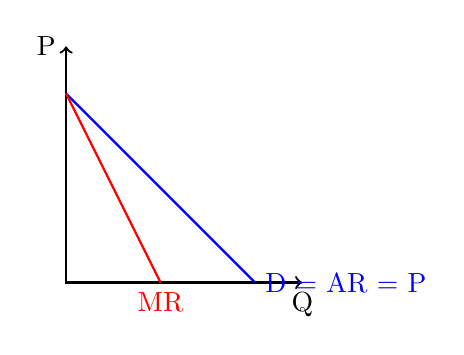
\begin{tikzpicture}[scale=0.6]
            \draw[thick, <->] (0,5) node[left]{P} -- (0,0) -- (5,0) node[below]{Q};
            \draw[blue, thick] (0,4) -- (4,0) node[right]{D = AR = P};
            \draw[red, thick] (0,4) -- (2,0) node[below]{MR};
        \end{tikzpicture}
        \end{center}
    \end{columns}
\end{frame}

\begin{frame}{Elasticity and Total Revenue}
    Monopolists maximize profit, not revenue, but they are constrained by demand elasticity.
    \vspace{0.3cm}
    \begin{itemize}
        \item \textbf{Elastic Range:} MR is positive ($MR > 0$). Lowering price increases Total Revenue (TR).
        \item \textbf{Unit Elastic:} MR is zero ($MR = 0$). TR is maximized.
        \item \textbf{Inelastic Range:} MR is negative ($MR < 0$). Lowering price decreases TR.
    \end{itemize}
    \vspace{0.3cm}
    \textbf{Key Rule:} A monopoly will \textbf{never} produce in the inelastic range (where $MR < 0$) because it lowers Total Revenue and increases costs.
\end{frame}

%===========================================================
\section{Profit Maximization}
%===========================================================

\begin{frame}{Graphing the Monopoly}
    \begin{columns}
        \column{0.4\textwidth}
        \textbf{The Golden Rule:}
        \begin{itemize}
            \item Produce where $MR = MC$.
        \end{itemize}
        \vspace{0.2cm}
        \textbf{Steps to Graphing:}
        \begin{enumerate}
            \item Find $Q$ where $MR = MC$.
            \item Go \textbf{up} to the Demand curve to find Price ($P_m$).
            \item Compare $P_m$ to ATC to find Profit/Loss.
        \end{enumerate}
        
        \column{0.6\textwidth}
        \begin{center}
        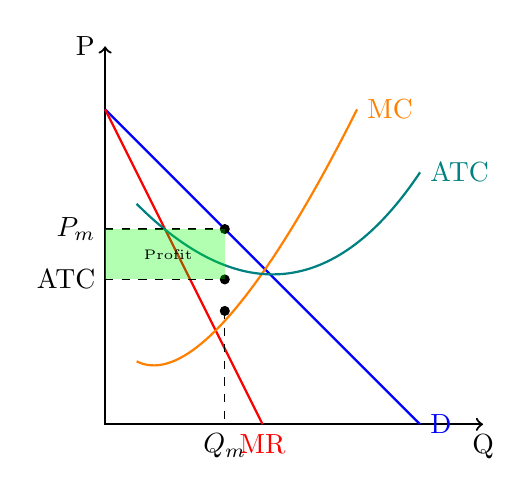
\begin{tikzpicture}[scale=0.8]
            \draw[thick, <->] (0,6) node[left]{P} -- (0,0) -- (6,0) node[below]{Q};
            
            % Demand and MR
            \draw[blue, thick] (0,5) -- (5,0) node[right]{D};
            \draw[red, thick] (0,5) -- (2.5,0) node[below]{MR};
            
            % MC and ATC
            \draw[orange, thick] (0.5,1) .. controls (1.5,0.5) and (3,3) .. (4,5) node[right]{MC};
            \draw[teal, thick] (0.5,3.5) .. controls (2.5,1.5) and (4,2.5) .. (5,4) node[right]{ATC};
            
            % Intersection MR=MC
            \filldraw (1.9, 1.8) circle (2pt) node[right, yshift=-5pt]{};
            \draw[dashed] (1.9, 1.8) -- (1.9, 0) node[below]{$Q_m$};
            
            % Price on Demand
            \filldraw (1.9, 3.1) circle (2pt);
            \draw[dashed] (0, 3.1) node[left]{$P_m$} -- (1.9, 3.1);
            
            % Cost on ATC
            \filldraw (1.9, 2.3) circle (2pt);
            \draw[dashed] (0, 2.3) node[left]{ATC} -- (1.9, 2.3);
            
            % Profit Box
            \fill[green, opacity=0.3] (0, 2.3) rectangle (1.9, 3.1);
            \node at (1, 2.7) {\tiny Profit};
        \end{tikzpicture}
        \end{center}
    \end{columns}
\end{frame}

\begin{frame}{Calculating Profit}
    \begin{block}{The Formula}
    $$ \text{Total Profit} = (P - ATC) \times Q $$
    \end{block}
    
    \begin{itemize}
        \item \textbf{Total Revenue (TR):} $P \times Q$
        \item \textbf{Total Cost (TC):} $ATC \times Q$
        \item \textbf{Per-Unit Profit:} $P - ATC$
    \end{itemize}
    \vspace{0.5cm}
    \textit{Tip: When answering graph questions, first locate MR=MC to find quantity, then go UP to Demand for price.}
\end{frame}

%===========================================================
\section{Inefficiency and Deadweight Loss}
%===========================================================

\begin{frame}{Monopolies and Efficiency}
    Unlike Perfect Competition, Monopolies are \textbf{inefficient}.
    
    \vspace{0.5cm}
    \begin{enumerate}
        \item \textbf{Not Allocatively Efficient:}
        \begin{itemize}
            \item Society wants $P = MC$.
            \item Monopoly produces where $P > MC$.
            \item Result: Underproduction (not enough resources allocated).
        \end{itemize}
        \vspace{0.2cm}
        \item \textbf{Not Productively Efficient:}
        \begin{itemize}
            \item Efficiency requires producing at minimum ATC.
            \item Monopoly produces where $P > \text{min ATC}$.
            \item Result: Higher costs than necessary.
        \end{itemize}
    \end{enumerate}
\end{frame}

\begin{frame}{Deadweight Loss (DWL)}
    \begin{columns}
        \column{0.5\textwidth}
        \textbf{Deadweight Loss:}
        \begin{itemize}
            \item The loss of consumer and producer surplus due to market inefficiency.
            \item Located \textbf{below} Demand, \textbf{above} MC, and to the \textbf{left} of the socially optimal quantity ($P=MC$).
            \item The shaded triangle points to the allocatively efficient quantity ($Q_{soc}$).
        \end{itemize}

        \column{0.5\textwidth}
        \begin{center}
        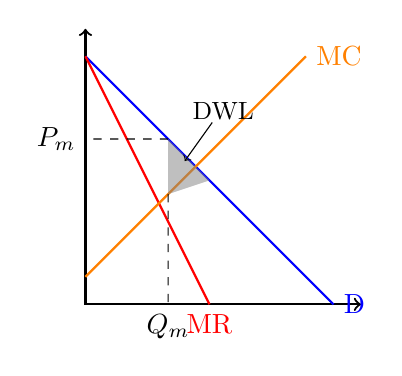
\begin{tikzpicture}[scale=0.7]
            \draw[thick, <->] (0,5) -- (0,0) -- (5,0);
            
            \draw[blue, thick] (0,4.5) -- (4.5,0) node[right]{D};
            \draw[red, thick] (0,4.5) -- (2.25,0) node[below]{MR};
            \draw[orange, thick] (0,0.5) -- (4,4.5) node[right]{MC};
            
            % MR = MC
            \coordinate (A) at (1.5, 2); 
            \draw[dashed] (A) -- (1.5, 0) node[below]{$Q_m$};
            
            % Price
            \coordinate (B) at (1.5, 3);
            \draw[dashed] (B) -- (0,3) node[left]{$P_m$};
            
            % Social Opt
            \coordinate (C) at (2.4, 2.9); % Approx intersection D and MC
            
            % DWL Triangle
            \fill[gray, opacity=0.5] (1.5, 2) -- (1.5, 3) -- (2.25, 2.25) -- cycle;
            \node at (2.5, 3.5) {\small DWL};
            \draw[->] (2.3, 3.3) -- (1.8, 2.6);
        \end{tikzpicture}
        \end{center}
    \end{columns}
\end{frame}

%===========================================================
\section{Price Discrimination}
%===========================================================

\begin{frame}{Price Discrimination}
    \textbf{Definition:} Charging different consumers different prices for the same product based on their willingness to pay (not based on cost differences).
    
    \vspace{0.3cm}
    \textbf{Conditions Required:}
    \begin{enumerate}
        \item Firm must have monopoly power (price maker).
        \item Firm must be able to segregate the market (identify elastic vs. inelastic customers).
        \item Consumers cannot resell the product (no arbitrage).
    \end{enumerate}
    \vspace{0.2cm}
    \textit{Examples: Movie tickets (matinee vs. evening), Airline tickets.}
\end{frame}

\begin{frame}{Perfect Price Discrimination Graph}
    If a monopoly practices \textbf{Perfect Price Discrimination}:
    \begin{columns}
        \column{0.5\textwidth}
        \begin{itemize}
            \item \textbf{D = MR}: The marginal revenue curve disappears; MR merges with Demand.
            \item \textbf{No Consumer Surplus}: Every consumer pays their exact maximum willingness to pay.
            \item \textbf{Higher Profits}: The profit area expands significantly.
            \item \textbf{Allocatively Efficient}: Surprisingly, they produce where $P=MC$, so there is no DWL!
        \end{itemize}
        
        \column{0.5\textwidth}
        \begin{center}
        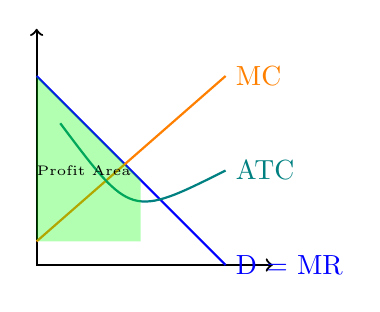
\begin{tikzpicture}[scale=0.6]
            \draw[thick, <->] (0,5) -- (0,0) -- (5,0);
            \draw[blue, thick] (0,4) -- (4,0) node[right]{D = MR};
            \draw[orange, thick] (0,0.5) -- (4,4) node[right]{MC};
            \draw[teal, thick] (0.5,3) .. controls (2,1) .. (4,2) node[right]{ATC};
            
            \fill[green, opacity=0.3] (0,0.5) -- (0,4) -- (2.2, 1.8) -- (2.2, 0.5) -- cycle;
            \node at (1, 2) {\tiny Profit Area};
        \end{tikzpicture}
        \end{center}
    \end{columns}
\end{frame}

%===========================================================
\section{Natural Monopolies \& Regulation}
%===========================================================

\begin{frame}{Natural Monopolies}
    \begin{itemize}
        \item A \textbf{Natural Monopoly} exists when economies of scale are so extensive that one firm can supply the entire market at a lower cost than two or more firms.
        \item \textbf{Key Graph Feature:} ATC is falling throughout the relevant range of production.
        \item \textit{Examples: Electricity, Water, Natural Gas (Utilities).}
    \end{itemize}
\end{frame}

\begin{frame}{Regulating Natural Monopolies}
    Governments regulate these monopolies to lower prices and increase efficiency.
    
    \begin{center}
    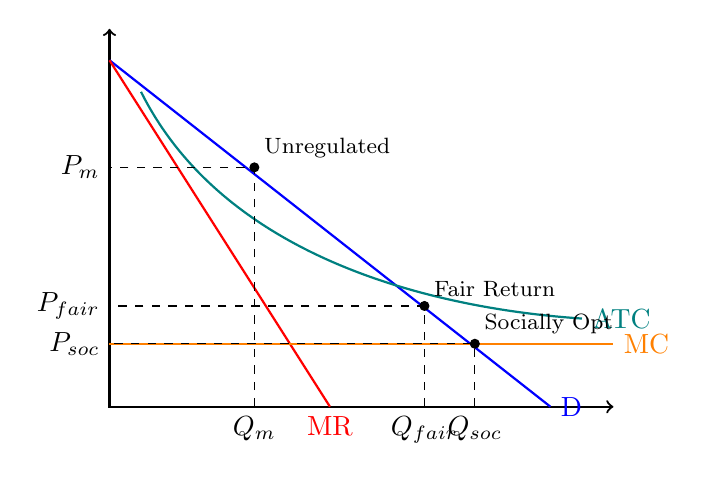
\begin{tikzpicture}[scale=0.8]
        \draw[thick, <->] (0,6) -- (0,0) -- (8,0);
        
        \draw[blue, thick] (0,5.5) -- (7,0) node[right]{D};
        \draw[red, thick] (0,5.5) -- (3.5,0) node[below]{MR};
        
        % Falling ATC and Low MC
        \draw[teal, thick] (0.5, 5) .. controls (2, 2) and (6, 1.5) .. (7.5, 1.4) node[right]{ATC};
        \draw[orange, thick] (0, 1) -- (8, 1) node[right]{MC};
        
        % Unregulated (MR=MC)
        \draw[dashed] (2.3, 0) node[below]{$Q_m$} -- (2.3, 3.8) -- (0, 3.8) node[left]{$P_m$};
        \filldraw (2.3, 3.8) circle (2pt) node[above right]{\footnotesize Unregulated};

        % Fair Return (P=ATC)
        \draw[dashed] (5, 0) node[below]{$Q_{fair}$} -- (5, 1.6) -- (0, 1.6) node[left]{$P_{fair}$};
        \filldraw (5, 1.6) circle (2pt) node[above right]{\footnotesize Fair Return};
        
        % Socially Optimal (P=MC)
        \draw[dashed] (5.8, 0) node[below]{$Q_{soc}$} -- (5.8, 1) -- (0, 1) node[left]{$P_{soc}$};
        \filldraw (5.8, 1) circle (2pt) node[above right]{\footnotesize Socially Opt};

    \end{tikzpicture}
    \end{center}
\end{frame}

\begin{frame}{Regulation Strategies Summarized}
    \begin{enumerate}
        \item \textbf{Unregulated Monopoly ($MR = MC$):}
        \begin{itemize}
            \item High price ($P_m$), low quantity ($Q_m$).
            \item Results in DWL.
        \end{itemize}
        
        \item \textbf{Socially Optimal Pricing ($P = MC$):}
        \begin{itemize}
            \item Allocatively efficient.
            \item Problem: In natural monopolies, $P < ATC$, causing a loss. The firm requires a subsidy to stay in business.
        \end{itemize}
        
        \item \textbf{Fair-Return Pricing ($P = ATC$):}
        \begin{itemize}
            \item Firm earns Normal Profit (Break-even).
            \item No subsidy needed.
            \item Less DWL than unregulated, but not perfectly efficient.
        \end{itemize}
    \end{enumerate}
\end{frame}

%===========================================================
\section{Review Formulas}
%===========================================================

\begin{frame}{Formulas to Remember}
    \begin{itemize}
        \item \textbf{Profit-Maximizing Rule:} $MR = MC$
        \item \textbf{Profit:} $(P - ATC) \times Q$
        \item \textbf{Total Revenue:} $P \times Q$
        \item \textbf{Total Cost:} $ATC \times Q$
        \item \textbf{Allocative Efficiency:} $P = MC$
        \item \textbf{Productive Efficiency:} $P = \text{minimum } ATC$
        \item \textbf{Fair Return Price:} $P = ATC$
    \end{itemize}
\end{frame}

\begin{frame}{End of Unit 5}
    \centering
    \Huge \textbf{Questions?}
\end{frame}

\end{document}
